%!TEX root = ../Hardtung_BA_SoSe20.tex

\section{Changes and new Features}
\label{sec:solutions}

This section will build on the discovered usability issues found during the initial evaluation process (see Section \ref{sec:evaluation}). On this basis, solutions can be developed that fix the most impactful usability issues. Furthermore, new features can be created that increase productivity (by automating processes and part of the workflow), while also fixing the current problems.


\subsection{Graphical User Interface related changes}

These changes include everything that is related to the graphical user interface that the user interacts with.

\subsubsection{Overall UI Changes}
Every feature area (e.g. grid options, scaling options, arrow/symbol inputs etc.) should be seperated through an \texttt{EtchedBorder} with its name as the title. Within these borders, elements should follow a consistent order. This is why this hierarchy is being set for the placement within these areas: \texttt{JRadioButton, JTextField, JButton, JCheckBox}.

Though additional \texttt{JLabels} can be used to explain or to give indicators what the elements do specifically. Whenever possible, icons should replace text and tooltips should be used to give further explanation. Explanatory \texttt{JLabels} should only be used when icons and tooltips are not enough.

Additionally, to the more consistent placement of elements within the UI, their sizes should be standardized as well. \texttt{JTextFields} for example should only be large enough to encapsulate the largest possible entry. This means that the \texttt{height} should always be set to 25 pixels (and the \texttt{width} depending on what is being entered (e.g. entering an angle between 0-360° will be shorter than entering the textual explanation of a folding step).
\newline
\textbf{Fixes: \#2.01; \#2.02; \#2.03; \#4.01; \#4.03}\\

\subsubsection{Side Panel}

The text of the \texttt{JRadioButtons} at the tool bar should be replaced by self-explanatory icons in order to improve overall clarity. But the textual explanation of all the tools should still be present to help especially novizes. This can be done through tooltips that appear when hovering over the buttons.

\noindent \textbf{Fixes: \#2.01; \emph{\#2.03}}
\newline

%Later Change
\noindent At a later point a complete redesign and rework of the UI will have to be carried out, in order to facilitate the goal of a unified and obstructionless design. At the current stage of development though the focus is being set to increase the efficiency and speed of creating origami diagrams.

\subsection{User Input related Changes}

\subsubsection{Arrows \& Symbols}
A large part of the Origrammer is made up of the different arrows and symbols that can be used in diagrams. So far, these objects were simple vector graphics that were being placed on the diagram as \texttt{ImageIcons} of \texttt{JLabels}. This approach did initially work, but brought restrictions and problems with it.

As vector graphics do not have explicit width or height values, the library Batik\footnote{\url{https://xmlgraphics.apache.org/batik/}}, which was being used to load the .svg files, presented wrong values to the \texttt{JLabel.setBounds(width, height)}-method. As a result of this limitation, the arrows \& symbols got partially cut off at the original bounds of the \texttt{JLabel} when rotating them. To fix this issue, a new, pre-rotated vector graphic was being loaded whenever an arrow or symbol got rotated. Though this in turn facilitated itself in a wrong, always square border around the arrows and symbols. Additionally, this made interactions with arrows and symbols far slower and unflexible.

\begin{figure*}[htbp]
	\centering
	\begin{subfigure}{0.3\textwidth}
		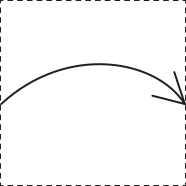
\includegraphics[width=\textwidth]{arrowLabelBorderStraight}
		\caption{Straight Arrow}
		\label{fig:arrowLabelBorderStraight}
	\end{subfigure}
	\begin{subfigure}{0.3\textwidth}
		\includegraphics[width=\textwidth]{arrowLabelBorderAngled}
		\caption{Angled Arrow}
		\label{fig:arrowLabelBorderAngled}
	\end{subfigure}
	\caption{Unwanted scaling when rotating\\ the wrong, always square hitbox, regardless of arrow shape}
	\label{fig:unwantedScaling}
\end{figure*}

\noindent Another sideeffect was a change in scale when rotating a non square object. A \texttt{JLabel} tries to display the biggest possible object that can fit within the border bounds. As seen on Figure \ref{fig:unwantedScaling} the size of the arrow changes after rotating it by 45°.

As a result of these problems and limitations, the decision was made to completely rework how arrows \& symbols function in the Origrammer. The new approach was to rebuild all objects with simple \texttt{java.awt.Shape}-objects. This gave total control over rotations, scaling, and on-the-fly-editing of all arrows/symbols. Another advantage was the removed reliance on \texttt{JLabels} and associated with that, there were no longer issues with wrong hitboxes or different scaling while rotating. The only disadvantage was the work-intensive nature of remodeling all arrows and symbols with \texttt{Shape}-objects by hand.
\newline
\textbf{Fixes: \#1.02; \#7.05; \#7.06}

\subsubsection{Dynamic Input Previews}

The Origrammer currently has 24 different lines, arrows, and symbols that can be placed, some of which require varying input sequences. This can be confusing for novices that are not familiar with the specific inputs. Because of this potential source of frustration, a dynamic preview was implemented for all lines, arrows, and symbols. This preview starts showing the object that is to be placed, before finalizing the placement.

As lines for example only require two mouse clicks to place, the preview can be shown after the first point of the line has been defined. Afterwards the line preview can show a line between the first point and the mouse cursor.

Objects like the rotation symbol that only require one mouse click for their placement, immediately show the symbol preview at the current mouse position.
\newline
\textbf{Fixes: \#1.01; \#1.02; \#3.01; \#6.02}

\newpage

\subsubsection{Filling Tool}

The current limitations of the Filling Tool make it slow and cumbersome to use. The user has to manually input three vertices in order to create a triangle that shows the specified filling color. The limit of only three vertices per \texttt{OriFace}-object was originally introduced to give finer control for the user, as well as simplifying the development process for this feature.

But this decision went against the original goal of minimizing the time needed to create diagrams. As a result the Filling Tool has to be reworked, so that it can be used faster and with less user inputs.

\begin{figure}[htbp]
	\centering
	\includegraphics[width=0.82\textwidth]{fillingToolExample}
	\caption{Example on how the Filling Tool works after the rework}
	\label{fig:fillingToolExample}
\end{figure}
\noindent The new Filling Tool only requires one mouse click to fill an area with colour. When clicking in an area, the Origrammer first looks for the closest line to the \texttt{clickPoint}. Afterwards, both endpoints of the line are being checked for other touching or intersecting lines. The additional lines that were found have to be checked if they are visible from the original \texttt{clickPoint}, which would mean, that they are part of the enclosing lines. The endpoints of every new discovered line will be checked the same way, until a full enclosure of lines is established. Once this has happened, a \texttt{GeneralPath} is created that goes through all points of the enclosing area. Lastly, the area of the \texttt{GeneralPath} can be filled with the specified colour.

%Finish explanations of how the Filling Tool works after the rework

\subsection{New Origrammer Features}

These new features should increase the productivity and efficiency of the Origrammer. The focus should be set on maximising the work that can be done in the shortest amount of time. This will be achieved by implementing features that either automate parts of the workflow, or that give new, faster possibilities of achieving the goal.

\subsubsection{Step Navigation \& Step Editing Options}

Currently, the Origrammer can create new diagram steps with three different options (\emph{Empty Step}, \emph{Copy last Step}, and \emph{Basic Paper Shape}). Furthermore, the user can navigate through them with a \emph{Next-Step}-/ and a \emph{Previous-Step}-button, though this approach brings limitation with it. Moving through the steps one by one hinders the overall usefulness and especially the speed of working with the Origrammer.

%delete and move and create in between
Deleting redundant steps can be quite important once the folding sequence goes through changes or simply when the user has made a mistake. In the same sense of offering solutions to user made mistakes, the Origrammer should make it possible to move steps to a different position within the diagram. Being able to create new steps in between existing ones can also be quite useful in negating user error.

%preview and make step active through clicking
An additional problem arises, once a diagram with a lot of steps (100+) is created. As the user currently only knows where he is in the folding sequence by the step number, this can lead to confusion. For example when folding an animal, there can be a different folding sequence, depending on what the artist decides to fold first (e.g. head first, the front or the hind legs, the tail, the abdomen, or the back). In order to continuously see where the user is within the diagram, there should be a small preview picture for all the steps within the step navigation. This will give the user an idea on what area a range of steps is working on. When clicking on one of the previews, the clicked step should made active and should be displayed on the Editing Panel.

As a result of the mentioned issues, the step navigation will be reworked to offer more functionality, visibility and ease of use. This will be accomplished by offering the following features in the rework:
\newpage
\begin{itemize}
\item Small preview picture of a step
\item Click on preview picture to show the step in the Editing Panel
\item Show step number, the preview picture, as well as the folding description of the step in the navigation
\item Delete a selected step
\item Move a selected step to the front or the back
\item Create a new step between existing steps
\end{itemize}

\textbf{Fixes: \#1.03; \#3.02;   \#7.07}

\subsubsection{Folding Presets}
In origami diagramming, there are eight widely established bases (Lang, 2012, p.53-64 \cite{DesignSecrets}). When starting with these bases, one can fold a variety of different models. The bases in question are:
 
 \begin{figure}[htbp]
	\centering
	\includegraphics[width=0.8\textwidth]{BasesTree}
	\caption[Family Tree of the standard bases.\\
	Top to bottom and left to right:  Cupboard Base, Windmill Base, Kite Base, Fish Base, Preliminary Fold, Bird Base, Waterbomb Base, Frog Base]{Family Tree of the standard bases.\\
	Top to bottom and left to right:  Cupboard Base, Windmill Base, Kite Base, Fish Base, Preliminary Fold, Bird Base, Waterbomb Base, Frog Base - (Robert J. Lang, 2011, p.61 \cite{BaseTree})}
	\label{fig:basesTree}
\end{figure}
\newpage
\noindent As these bases serve as the starting point for a wide array of models, it would be helpful to include them in the Origrammer. By giving the user the option to start a diagram with one of these bases, the overall diagramming process will be shortened by quite a bit. Not having to keep repeating the same beginning steps for different models will save time and can also show beginners of the program, how parts of the Origrammer look like or work.

Additionally to the origami bases, instructions on how to fold different grid sizes, should be included in the folding presets as well. Folding a 3x3, 5x5, or 7x7 grid from a square paper is not as straight forward and requires multiple folding steps to achieve. 

 \begin{figure}[h]
	\centering
	\includegraphics[width=1.1\textwidth]{5x5-grid}
	\caption{Example diagram of a 5x5 grid made with the Origrammer}
	\label{fig:5x5-grid}
\end{figure}

\textbf{Fixes: \#7.09}

\newpage
\subsubsection{Additional Line Input Types}

So far lines in the Origrammer could only be inputted at existing vertices or through the helping grid. In order to give the user more flexibility and control more line input variants have been implemented.\\
\newline
\noindent \textbf{Angle Bisector}\\
\noindent In case an angle has to be folded in half, the user can now use the \emph{Angle Bisector} line input. The two lines that span the angle that is to be folded in half have to be selected and the Origrammer automatically places this new crease line.\\
\newline
\noindent \textbf{Perpendicular}\\
\noindent Often times crease lines will be placed at irregular angles and this feature makes it possible to create perpendicular (90°) lines at any existing line. This perpendicular line is extended until it hits an existing line. Its direction can be reversed when holding the \emph{CTRL}-key during line input.\\
\newline
\noindent \textbf{Extend Line}\\
\noindent On occasion important reference points are missing and make some lines impossible to input. The \emph{Extend Line} feature works by inputting a normal line through the existing reference points and the grid, but then the line gets extended to both sides until it crosses other existing lines.\\
\newline
\noindent \textbf{Mirror Lines}\\
\noindent Origami models often times have mirrored sides and thus a \emph{Mirror Lines} feature was introduced. First, the user selects  the lines that should be mirrored. After that a mirror line has to be specified, which will be the line where all selected lines will be mirrored from.\\
\newline
\noindent \textbf{By Length and Angle}\\
\noindent Placing lines with a specific angle (towards the x-axis) and length gives the user even more fine control over line placement. This input method can be combined with the \emph{Measure Angle/Length}-tool in order to copy existing lines.

\textbf{Fixes: \#3.04}